%Srinivas Vaidyanathan - 130010033
\documentclass[12pt,a4paper]{report}
\usepackage{hyperref}
\usepackage{color}
\usepackage{graphicx}
\usepackage{cite}
\begin{document}
\bibliographystyle{plain}
\hypersetup{pageanchor=false}
\title{Analysis Of An LC Tank With Resistance}
\author{Srinivas Vaidyanathan \\ 130010033 Aerospace Engineering}
\maketitle
\hypersetup{pageanchor=true}
\begin{abstract}
  This report contains an analysis of an LC circuit with a resistance connected in series.
  The variation current flowing through the LCR circuit and the charge in the capacitor have been studied.
  The code to generate the plots for this report is present in \textcolor{blue}{\url{https://github.com/srinivasv147/LCR}}.
  The code in the said repository requires python 2.7 to be installed in the
  machine. Also, the code for generating the report in pdf format has been tested only with MacTex-2016.
\end{abstract}
\hypersetup{pageanchor=false}
\section{Circuit description and analysis}
Figure \ref{fig:circuit} shows the circuit we are about to analyse ~\cite{mit:pres}.
\begin{figure}[h!]
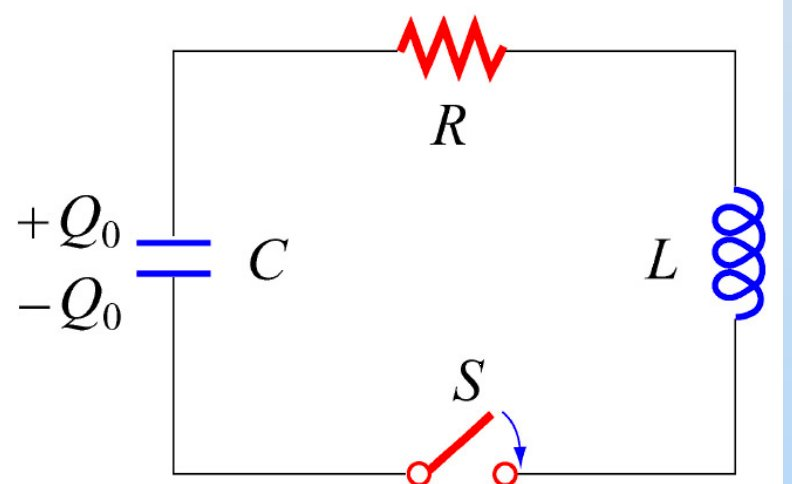
\includegraphics[width=\linewidth]{lcr.jpg}
\caption{The LCR circuit (130010033)}
\label{fig:circuit}
\end{figure}\\
The circuit consists of an inductor of inductance L, a capacitor of capacitance C and a resistance of resistance R.
We start By applying the Kirchhoff's Voltage rule across the circuit. This gives us the following expression ~\cite{wiki:LCR}.
\begin{equation}
L\frac{dI}{dt}+\frac{Q}{C}+IR=0
\label{init:equation}
\end{equation}
Also seeing that the charge in the capacitor $Q_0=\int{Idt}$ we can modify equation \textcolor{blue}{\ref{init:equation}} as
\begin{equation}
L\frac{dI}{dt}+\frac{1}{C}\int{Idt}+IR=0
\label{mod:equation}
\end{equation}
Now if we differentiate both sides of the equation \textcolor{blue}{\ref{mod:equation}} with respect to time we get:
\begin{equation}
L\frac{d^2I}{dt^2}+R\frac{dI}{dt}+\frac{1}{C}=0
\label{def:equation}
\end{equation}
dividing both sides of equation \textcolor{blue}{\ref{def:equation}} with L we get:
\begin{equation}
\frac{d^2I}{dt^2}+\frac{R}{L}\frac{dI}{dt}+\frac{1}{LC}=0
\label{findef:equation}
\end{equation}
The equation \textcolor{blue}{\ref{findef:equation}} is of the form of the standard second order system which
is of the form:
\begin{equation}
\frac{d^2x}{dt^2}+2\xi \omega_n\frac{dx}{dt}+\omega_n ^2=0
\label{std:equation}
\end{equation}
Comparing coefficients with the equation \textcolor{blue}{\ref{std:equation}} we get:
\begin{equation}
2\xi\omega_n=\frac{R}{L}
\label{comp1:equation}
\end{equation}
\begin{equation}
\omega_n ^2=\frac{1}{C}
\label{comp2:equation}
\end{equation}
From equations \textcolor{blue}{\ref{comp1:equation}} and \textcolor{blue}{\ref{comp2:equation}} we get:
\begin{equation}
\xi=\frac{R}{2}\sqrt{\frac{C}{L}}
\label{compres1:equation}
\end{equation}
\begin{equation}
\omega_n=\frac{1}{\sqrt{LC}}
\label{compres2:equation}
\end{equation}
The general solution to the equation \textcolor{blue}{\ref{std:equation}} is given as:
\begin{equation}
x=e^{-\xi\omega_nt} [Ae^{t\omega_n\sqrt{\xi^2 - 1}}+Be^{-t\omega_n\sqrt{\xi^2 - 1}}]
\label{sol:equation}
\end{equation}
Where A and B are constants dependant on the initial conditions.Here we assume A and B as constants
and study the behaviour of the circuits at different values of RLC in terms of A and B.\\ From the equation
\textcolor{blue}{\ref{sol:equation}} there are only 3 main classes of solutions i.e. $0<\xi<1$, $\xi=1$, $\xi>1$
and in terms of circuit parameters $R^2<\frac{4L}{C}$, $R^2=\frac{4L}{C}$, $R^2>\frac{4L}{C}$. The plots for
these cases are shown below. The video link is  \textcolor{blue}{\href{run:./plots130010033_eta=0.5.mp4}{here}}
\begin{figure}[ht!]
\includegraphics[width=\linewidth]{plots.png}
\caption{The current vs time plot (130010033)}
\label{fig:plot}
\end{figure}
\bibliography{sources}
\end{document}
